\begin{document}

\title{\ZHH \Huge 单点服务与热备机制}
\author{\small gaccob}
\date{\small 2014 年 3 月 8 日}
\maketitle

\section* {\Large \ZHH 一. 逻辑层的单点服务} {
    {在游戏业务中,一般都会尽量避免单点服务的存在,但是难免会有些特例,特别是全区全服的游戏中,由于一些业务的特性,很难做成分布式。例如排行榜服务,提供top的排名查询和更新;例如维护目录等meta信息的单master节点;例如提供创建名字和改名的name service等。这些业务可以提炼出一些共性:}
    \begin{enumerate}
    \item{提供读写服务,基本都有cache,数据变更会通过触发机制(定时或者消息触发)落地到存储层。}
    \item{逻辑比较简单,可靠性比较高,性能也一般不会成为整个系统的瓶颈。}
    \item{因为是单点的存在,会有因为机器故障而无法服务的风险。}
    \item{一般不会是关键业务,在服务不可用时可以有一定的容忍度。}
    \end{enumerate}\par

    {其实,这些服务大部分都是cache,可以通过直接对db操作来获得同样的结果,放在在逻辑层来做,是为了更简单的逻辑和更高的性能。}\par
    {基于上面的第3点,服务成为了单点,就会因为可靠性(high availability)带来做热备的需求。一般来说,热备都是存储或者硬件层面做的事情,很少会在逻辑层做,因为这会使得本来简单的逻辑和结构变复杂,增大系统的熵。}\par
    {这里需要做一定的妥协,anyway,架构设计本来就是一个平衡设计,在可用性、可扩展性、可维护性、可靠性、高性能等之间做妥协选择。个人认为:}\par
    \begin{itemize}
    \item{其一,如果能通过监控+脚本的自动化方式在可控的时间内恢复服务,不做热备。}
    \item{其二,如果直接忽略该服务,直接读写存储层,在性能以及逻辑的复杂度上可以接受,则抛弃之。}
    \item{其三,使用单点服务,同时为此买单做热备机制,是最后选择。}
    \end{itemize}
}


\section* {\Large \ZHH 二. 热备相关技术} {
    \subsection* {1. RAID 1} {
        {具体可以参考\href{http://zh.wikipedia.org/wiki/RAID#RAID_1}{wiki}。}\par
        {RAID 1是硬件层的备份方案,两组磁盘相互镜像,只要一组磁盘正常即可维持工作。如下图所示,假设disk 0是master,disk 1是slave,写磁盘操作是master和slave的双写,理论上读磁盘操作可以通过分布到master和slave上来获取性能的提升,但是一般还是只读master,只有当master故障时才切换到slave,同时给出告警。}\par
        \begin {figure}[htbp]
            \centering
            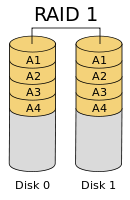
\includegraphics [width=100pt, keepaspectratio] {raid_1.png}
        \end {figure}
    }

    \subsection* {2. MySQL replication机制}{
        {MySQL提供了replication机制,它本身不是热备方案,只是一个数据同步的机制,本质是binary log同步。可以参考:\href{http://dp.imysql.com:8080/taxonomy/term/23}{《MySQL Replication/复制/同步》}.}\par
        {在master-slave的架构下,master服务器把更新的内容写到二进制日志binary log中,这些日志中的更新部分会被发送到slave服务器(可以是多个)。slave连接到master之后,从master拉取最新的增量更新操作数据。}\par
        {对于访问MySQL的业务来说,master可读写,slave只读,对于读写比大的业务来说能提升不少性能。另外还有master-slaves-slaves架构和master-master-slaves架构,具体的就不在这里阐述了。}\par
        {MySQL replication机制能够保证了在master故障时,slave被切换为master时,能迅速的恢复服务:数据基本不会丢(除了故障发生时那一刻的修改无法保证)。}\par
        {一般会使用MySQL replication,加上HA技术,自动化脚本,或者一些人工干预的手段来做热备方案。}\par
        \begin {figure}[htbp]
            \centering
            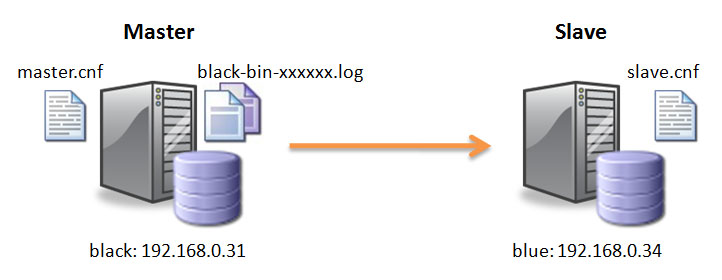
\includegraphics [width=300pt, keepaspectratio] {mysql_master_slave.jpg}
        \end {figure}
    }

    \subsection* {3. Linux HA 技术}{
        {HA(high availability)技术的关注点在集群中故障节点检测,以及在故障发生时的重新配置,从而实现服务不中断。}\par
        {节点的同步,则不在HA的范畴内,如果节点是有状态的,需要节点自己解决同步的问题,譬如上文中的MySQL replication。}\par
        \begin {figure}[htbp]
            \centering
            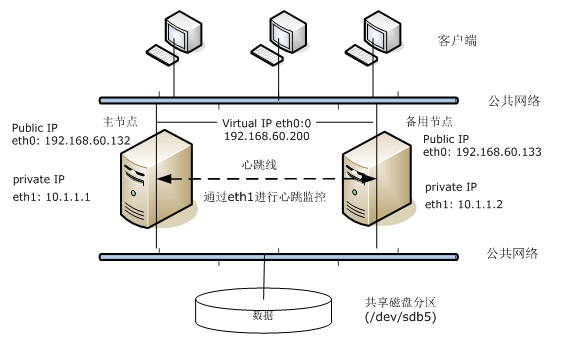
\includegraphics [width=300pt, keepaspectratio] {heartbeat_ha.png}
        \end {figure}
        {以典型的LVS负载均衡为例,LVS均衡器成为了单点,通过heartbeat加ldirector实现热备方案:heartbeat分别部署在LVS均衡器的master节点和slave节点上,通过串行线、以太网接口,或者同时使用两者,来检测对方的健康状态。一旦slave检测到master不可用,则自动接管master的资源,接管的过程一般通过ldirector配置相同的virtual ip实现。}\par
    }

    \subsection* {4. XFS master 主备方案}{
        {具体可以参考腾讯大讲堂文章: \href{http://djt.qq.com/article/view/322}{《XFS master主备机制》}}\par
        {这是一个真正完善成熟的主备方案,工作在应用层。XFS master节点以不同的角色(primary,secondary,newbie)运行多份,主master由zookeeper选举得到,master之间通过三套子协议:replication,failover,learning协作,完成同步工作,具备高可靠性,同时兼顾了性能。}\par
        \begin {figure}[htbp]
            \centering
            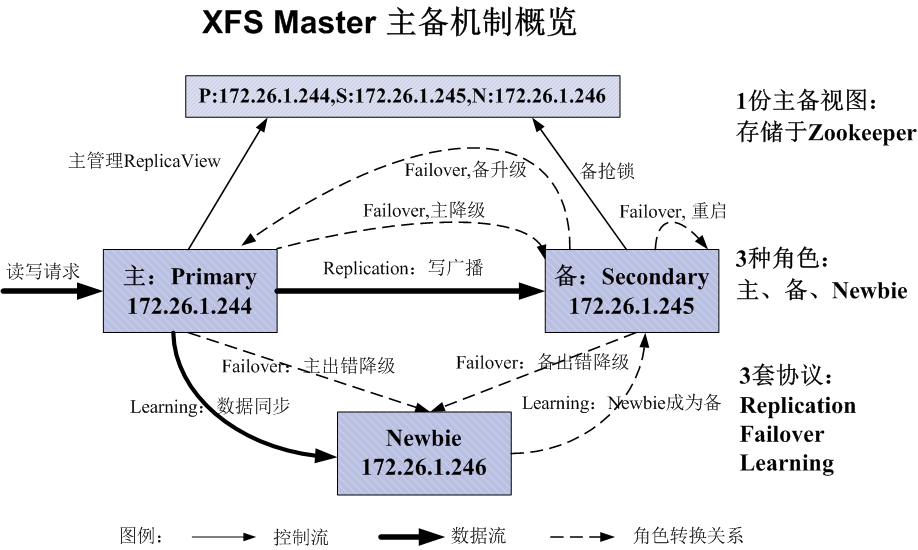
\includegraphics [width=300pt, keepaspectratio] {xfs_master.png}
        \end {figure}
    }
}


\section* {\Large \ZHH 三 总结与分析} {
    {简单总结归纳一下,完整的主备方案应该是这样:}\par
    \begin{enumerate}
    \item{需要一个{\color{red}监控者}:检验master节点故障.}
    \item{需要一个{\color{red}执行者}:在master节点故障之后,切换到slave机器.}
    \item{如果节点是有状态的,还需要一个{\color{red}传输者}:同步master的状态到slave.}
    \end{enumerate}\par

    {结合上一节中给出的热备技术或者方案来具体分析一下:}\par
    \begin{enumerate}
    \item{RAID 1的方案,监控者和执行者都是硬件直接搞定,传输者其实也是硬件实现的(写磁盘时的双写机制),所以也是一个比较完整的热备方案。}
    \item{MySQL replication机制,其实只是一个同步机制,充当着传输者的角色。}
    \item{Linux HA技术中,以上文中LVS集群为例,heartbeat既是监控者,又是执行者,不过这个执行者光吆喝,事情还得靠小弟(ldirector)来做。而且作为监控者,slave检查master是否故障,总觉得没那么靠谱,如果master与slave中间的心跳通信中断,是不是会带来比较复杂的情况?}
    \item{XFS的主备方案很完善,zookeeper集群是第三方的监控者和执行者,同时replication,failover,learning三套协议的交互,保证了master状态的同步,从而能在热备切换时迅速的恢复服务。但是同时,这也是最复杂的实现,方案的完备程度是与复杂度成正比的。}
    \end{enumerate}
}


\section* {\Large \ZHH 四 过往案例反思} {

    \subsection* {1. 单点namesvr的热备} {
        {刚入职时,做过的第一个独立模块就是name server,因为一些业务需求,不太容易根据号段来做分布,同时为了减少数据库事务,在本身数据量不大的情况下,做成了全量cache。因为是单点,所以为之做了热备的,简单的拓扑示意图如下:}
        \begin {figure}[htbp]
            \centering
            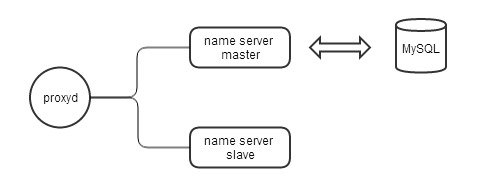
\includegraphics [width=300pt, keepaspectratio] {name_server.jpg}
        \end {figure}
        \begin {itemize}
            \item{proxyd是一个类似TSF4G组建中tbusd的角色,维护了通信关系。同时,这里的proxyd是name server热备方案的监控者与执行者,当监控到master故障时,会指挥slave切换,使之完成角色转换,切为master。}
            \item{name server知道自己当前的角色是master还是slave,如果是slave的话,仅仅操作cache,无需落地到MySQL(当然最开始的cache是程序启动时加载MySQL数据建立的)。}
            \item{name server本身是有状态的,所以还需要一个状态传输者,这里处理的方式做了一下迂回:因为name server的数据源都源自proxyd转发过来,所以proxyd对name server做了广播,间接保证了master和slave的状态一致。这里还有个前提,name server知道自己是master还是slave,如果是slave,不应该响应回包,不应该将数据落地到存储。最后,为了校验master和slave的状态一致性,定时的比对双方的流水日志,并以master为准。}
        \end {itemize}
        \par
        {现在回头再反思这个模块,会发现有很多的不合理之处,是个比较差的设计,这个模块在跑了一年多之后,据了解也确实被优化和重构了。}\par
        \begin{itemize}
            \item{首先,这里的name server应该可以通过一些方式,规避掉单点的设计,利用存储层DB的事务性,做成无状态的服务,从而简化整个架构。}
            \item{其次,在这里,proxyd扮演的角色太过复杂,既是通信的传输节点,又是热备方案的监控者和执行者,还参与了name server状态同步的传输过程。耦合度太高,违背了unix的精神。}
            \item{最后,状态同步用了比较迂回的方式,同时为了验证状态的一致,又引入了脚本检测机制,让事情变得愈加复杂。也许参考MySQL的bin-log同步是不错的方式,因为本身有流水日志的存在。}
        \end{itemize}
    }

    \subsection* {2. 配置中心center的热备} {
        {最近在工作中碰到的一个例子:这里的center有点类似XFS中的master,是一个路由配置中心,接受通信节点proxy的注册与查询,同样是一个单点。}\par
        {但是有一定的业务特性:在整个系统正常运作之后,只有通信端点的变更,才会有逻辑处理,所以做热备方案,在slave切换故障master时,可以相对容忍比较高的延迟。 这里的center热备方案是同事实现的,这里借花献佛拿出来分享一下。 } \par
        \begin {figure}[htbp]
            \centering
            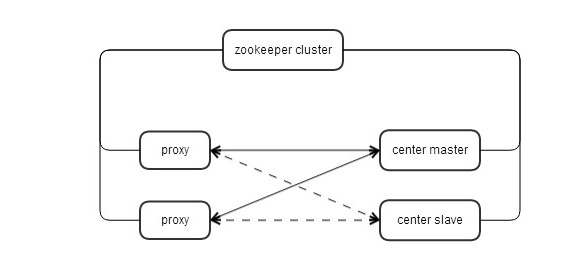
\includegraphics [width=300pt, keepaspectratio] {center.jpg}
        \end {figure}
        \begin{itemize}
            \item{center的master和slave都启动,并注册到zookeeper集群上。Zookeeper作为热备方案的监控者和执行者,当center master故障时,zookeeper能知道,并推选出新的master。}
            \item{在slave的切换过程中,有状态的同步过程的,不过是通过重新跑一遍逻辑来完成。 proxy在zookeeper上注册观察者身份,观察center的变更,当收到zookeeper消息,知道center master变更时,建立连接到新的master,并开始一系列重新注册的工作,重新建立配置关系,即所谓center的状态(这些都不影响正常的通信状态),而且这个过程不会太长,一般在秒级别。当center master的配置关系完全建立成功之后,center就已经恢复正常服务了。}
        \end{itemize}
        \par
        {与XFS类似,引入了第三方zookeeper来作为监控者和协调者,但是没有像XFS一样,使用多个角色及多套协议来做状态的同步:因为center作为非关键路径,是可以容忍一定程度的恢复延迟,所以这里舍弃了如bin-log,或者XFS的同步协议这些复杂的设计实现,保持了逻辑的简单。}\par
        {个人觉得这是一个很不错的设计,唯一的遗憾,在于zookeeper对于整个后台架构来说,略显重了一些。}\par
    }
}


\section* {\Large \ZHH 五 结束语} {
    {在业务逻辑层,最好的热备方案,就是没有单点,无需热备。}\par
    {没有绝对万能的架构,只有根据合适的场景做平衡设计,如何妥协是一门艺术。}\par
    {最后,借Allen的一句话:我所说的,都是错的。}\par
}

\end{document}
